\section{Checking Linearizability By Recursive Procedure}
\label{sec:checking linearizablity by recursive procedure}

In this section, we extend $\textit{check-PQ}$ with linearizability, and use it to simplify checking linearizability w.r.t $\textit{PQ}$. This inspired us to partition the concurrent executions which are not linearizable w.r.t $\textit{PQ}$ into violation of $\textit{MS}(R)$. To ensure the correctness of $\textit{check-PQ}$, we step-by-step linearizability to incrementally build linearization. Our step-by-step linearizability is inspired by the step-by-step linearizabilility of queue and stacks in \cite{Bouajjani:2015}. The related definitions and proofs of lemmas in this section can be found in Appendix \ref{sec:appendix in section step-by-step linearizability of extended priority queues}.


\subsection{Linearizability}
\label{subsec:linearizability}

A (concurrent) execution $e$ is a sequence of call and return actions which satisfy a well-formedness property: every return has a matching call action before it in $e$, and an operation $o$ can be used only twice in $e$, once in a call action, and once in a return action. The definition of data-differentiated, renaming function, data-independence and projection extends to (concurrent) executions. For instance, an execution is data-differentiated if, for all $d \in \mathbb{D}$, there is at most one $\textit{cal}_{\_}(\textit{put},d,\_)$.


Given execution $e$, the happen-before relation $<_{\textit{hb}}$ is defined as follows: $o_1 <_{\textit{hb}} o_2$, if the return action of $o_1$ is before the call action of $o_2$ in $e$. The happens-before relation are interval orders \cite{Bouajjani:2015POPL}: for distinct $o_1,o_2,o_3,o_4$, if $o_1 <_{\textit{hb}} o_2$ and $o_3 <_{\textit{hb}} o_4$, then either $o_1 <_{\textit{hb}} o_4$, or $o_3 <_{\textit{hb}} o_2$. Intuitively, this comes from the fact that concurrent threads share a notion of global time.

Linearizability \cite{Herlihy:1990} is the \emph{de facto} standard correctness condition for concurrent data structures. Given concurrent execution $e$ and sequential execution $s$ of length $n$, we say that $e$ is linearizable w.r.t $s$, denoted $e \sqsubseteq s$, if they have same set of operations, and there is a bijection $f$ between operations s.t.

\begin{itemize}
\item[-] if $o_1 <_{\textit{hb}} o_2$, then $f(o_1) <_{\textit{hb}} f(o_2)$,

\item[-] $o$ and $f(o)$ have same call and return actions.
\end{itemize}

A concurrent execution $e$ is linearizable w.r.t a set $S$ of sequential executions, denoted $e \sqsubseteq S$, if there exists $s \in S$ such that $e \sqsubseteq s$. A set of concurrent executions $E$ is linearizable w.r.t $S$, denoted $E \sqsubseteq S$, if $e \sqsubseteq S$ for all $e \in H$.

The following lemma states that with the help of data-independence, it is enough to consider only data-differentiated executions when checking linearizability. This is similar to that in \cite{Abdulla:2013}, where they use the notion of data-independence in \cite{Wolper:1986}. Thus, in the remainder of the paper, we focus on characterizing linearizability for data-differentiated executions. The proof of this lemma can be found in Appendix \ref{sec:appendix in section data-independence of EPQ}.

\begin{restatable}{lemma}{DataDifferentiatedisEnoughforPQ}
\label{lemma:data differentiated is enough for PQ}
A data-independent implementation $\mathcal{I}$ is linearizable w.r.t data-independent set $S$ of sequential executions, if and only if $\mathcal{I}_{\neq}$ is linearizable with respect to $S_{\neq}$.
\end{restatable}




\subsection{Modified $\textit{check-PQ}$}
\label{subsec:recursive procedure con-check-EPQ}

Let us extend $\textit{check-PQ}$ with linearizability to deal with linearizability w.r.t $\textit{PQ}$ as follows: 

\begin{itemize}
\setlength{\itemsep}{0.5pt}
\item[-] The input $e$ is a concurrent execution. 

\item[-] $\textit{last}(e)$ is the union of $\textit{last}(u)$ for any sequential execution $u$ such that $e \sqsubseteq u$. $e \sqsubseteq \textit{MS}(R)$ with witness $x$ (resp., $o$), if $e \sqsubseteq u \in \textit{MS}(R)$ and $x$ (resp., $o$) is the witness of $u$. 
    
\item[-] $P_i(e,o)$ and $P_i(e,x)$ holds, if $e \sqsubseteq \textit{MS}(\textit{PQ}_i)$ withe witness $o$ or $x$, respectively. 
\end{itemize} 

The following lemma states that $\textit{check-PQ}$ is correct. 

\begin{restatable}{lemma}{ConCheckEPQIsCorrect}
\label{lemma:con-check-EPQ is correct}
Given a data-differentiated execution $e$, $e \sqsubseteq \textit{EPQ}$, if and only if, $\textit{check-PQ} = \textit{true}$.
\end{restatable} 

\begin {proof} (Sketch)
It is not hard to see that $\textit{check-PQ}(e) = \textit{false} \Rightarrow e \not\sqsubseteq \textit{PQ}$, since $\textit{PQ}_{\neq} \subset \textit{MS}(R)_{\neq}$. To ensure that $\textit{check-PQ}(e) = \textit{true} \Rightarrow e \sqsubseteq \textit{PQ}$, we require $\textit{PQ}$ to satisfy the following property.  

for any data-differentiated execution $e$,
\begin{itemize}
\setlength{\itemsep}{0.5pt}
\item[-] if $e \sqsubseteq \textit{MS}(R)$ ($R \in \{ \textit{PQ}_1, \textit{PQ}_2 \}$) with witness $x$, we have: $e \setminus x \sqsubseteq \textit{PQ} \Rightarrow e \sqsubseteq \textit{PQ}$.

\item[-] if $e \sqsubseteq \textit{MS}(\textit{PQ}_3)$ and $o$ is a $\textit{rm}(\textit{empty})$, we have: $e \setminus o \sqsubseteq \textit{PQ} \Rightarrow e \sqsubseteq \textit{PQ}$.
\end{itemize}

With this property, we can build a linearization of a whole execution by increasingly construct linearization of sub-execution from $\epsilon$, and this convince us that $\textit{check-PQ}(e) = \textit{true} \Rightarrow e \sqsubseteq \textit{PQ}$. 

Let us briefly explain the idea of proving this property for $\textit{PQ}_1$ with an example. Given a data-differentiated concurrent execution $e \sqsubseteq u \cdot \textit{put}(x,p) \cdot v \cdot \textit{rm}(x) \cdot w \in \textit{MS}(\textit{PQ}_1)$ with witness $x$ and assume that $e \setminus x \sqsubseteq l' \in \textit{PQ}$, as shown in \figurename~\ref{fig:concurrent execution for EPQ1} (a), we explicitly construct a sequence $l''= l''_1 \cdot \textit{put}(x,p) \cdot l''_2 \cdot \textit{rm}(x) \cdot l''_3$ and prove that $e \sqsubseteq l'' \in \textit{PQ}$. In this example, $p_1 \prec p$, $p_1 \prec p_2$, $u=\epsilon$, $w$ contains $\textit{rm}(z_2), \textit{put}(x_3,p_2), \textit{rm}(z_1)$ (emphasize by $\textit{rm}(z_2)-w$), and the remanning operations are in $v$. We also explicitly draw the linearization points according to $l'$. We construct $l''$ as follows, and this method does not rely on the locations of linearization points of $l'$ and operations of $x$. Here we implicitly mix operation $o$ (when $\textit{call}_o(m,a)$, $\textit{ret}_o(m,b)$ in $e$) with $m(a,b)$.

\begin{itemize}
\setlength{\itemsep}{0.5pt}
\item[-] Let $p$-comparable operations (resp., $p$-incomparable operations) be the set of operations with items whose priority is comparable with $p$ (resp., incomparable with $p$). It seems that we can construct $l''_1$, $l''_2$ and $l''_3$ as the projection of $l'$ into operations of $u$, $v$ and $w$, respectively. However, this is incorrect, since $\textit{PQ}_1$ has no restriction to $p$-incomparable operations operations in $u \cdot v$, and thus, there is no guarantee that the projection of $l'$ into $p$-incomparable operations operations in $u \cdot v$ being correct. In this example, such projection is $\textit{put}(z_1,p_3) \cdot \textit{rm}(z_2)$ and is incorrect.

\item[-] Let us construct sets $U'$, $V'$ and $W'$, such then make $l''_1$, $l''_2$ and $l''_3$ the projections of $l'$ into $U'$, $V'$ and $W'$, respectively. This contains two steps:

\item[-] The first step is to define $W'$. The $p$-comparable operations in $W'$ is same as that in $w$. To obtain $p$-incomparable operations in $W'$, we try to find a $p$-incomparable operation $o$ which either happens before some $p$-comparable operations in $w$, or with linearization points after $\textit{rm}(x)$. Then, we put $o$ and all $p$-incomparable operations after $o$ in $l'$ into $W'$ (emphasized by boxes in example). In this example, $o$ is $\textit{rm}(z_1)$, and $W'$ contains $\textit{put}(x_3,p)$, $\textit{rm}(z_1)$ and $\textit{rm}(z_2)$. We use boxes to emphasize they are put into $W'$.

\item[-] The second step is to define $U'$ and $V'$. $U'$ contains the following two kinds of operations: (1) Operations whose linearization points are before $\textit{ret}(\textit{put},x)$, and (2) other $\textit{put}$ operations with priority $p$. $V'$ contains the remanning operations. In this example, $U'$ contains $\textit{put}(z_1,p_3)$ and $\textit{put}(x_2,p_2)$.

\item[-] In this example, $l''_1 = \textit{put}(z_1,p_2) \cdot \textit{put}(x_2,p)$, $l''_2 = \textit{put}(z_2,p_2) \cdot \textit{rm}(x_2) \cdot \textit{put}(y_1,p_1) \cdot \textit{rm}(y_1)$, and $l''_3 = \textit{put}(x_3,p) \cdot \textit{rm}(z_1) \cdot \textit{rm}(z_2)$. In \figurename~\ref{fig:concurrent execution for EPQ1} (b), we add linarization points according to $l''$, and we can see that $l''$ holds as required.
\end{itemize}

This completes the proof of this lemma. 


\qed
\end {proof}



\begin{figure}[htbp]
  \centering
  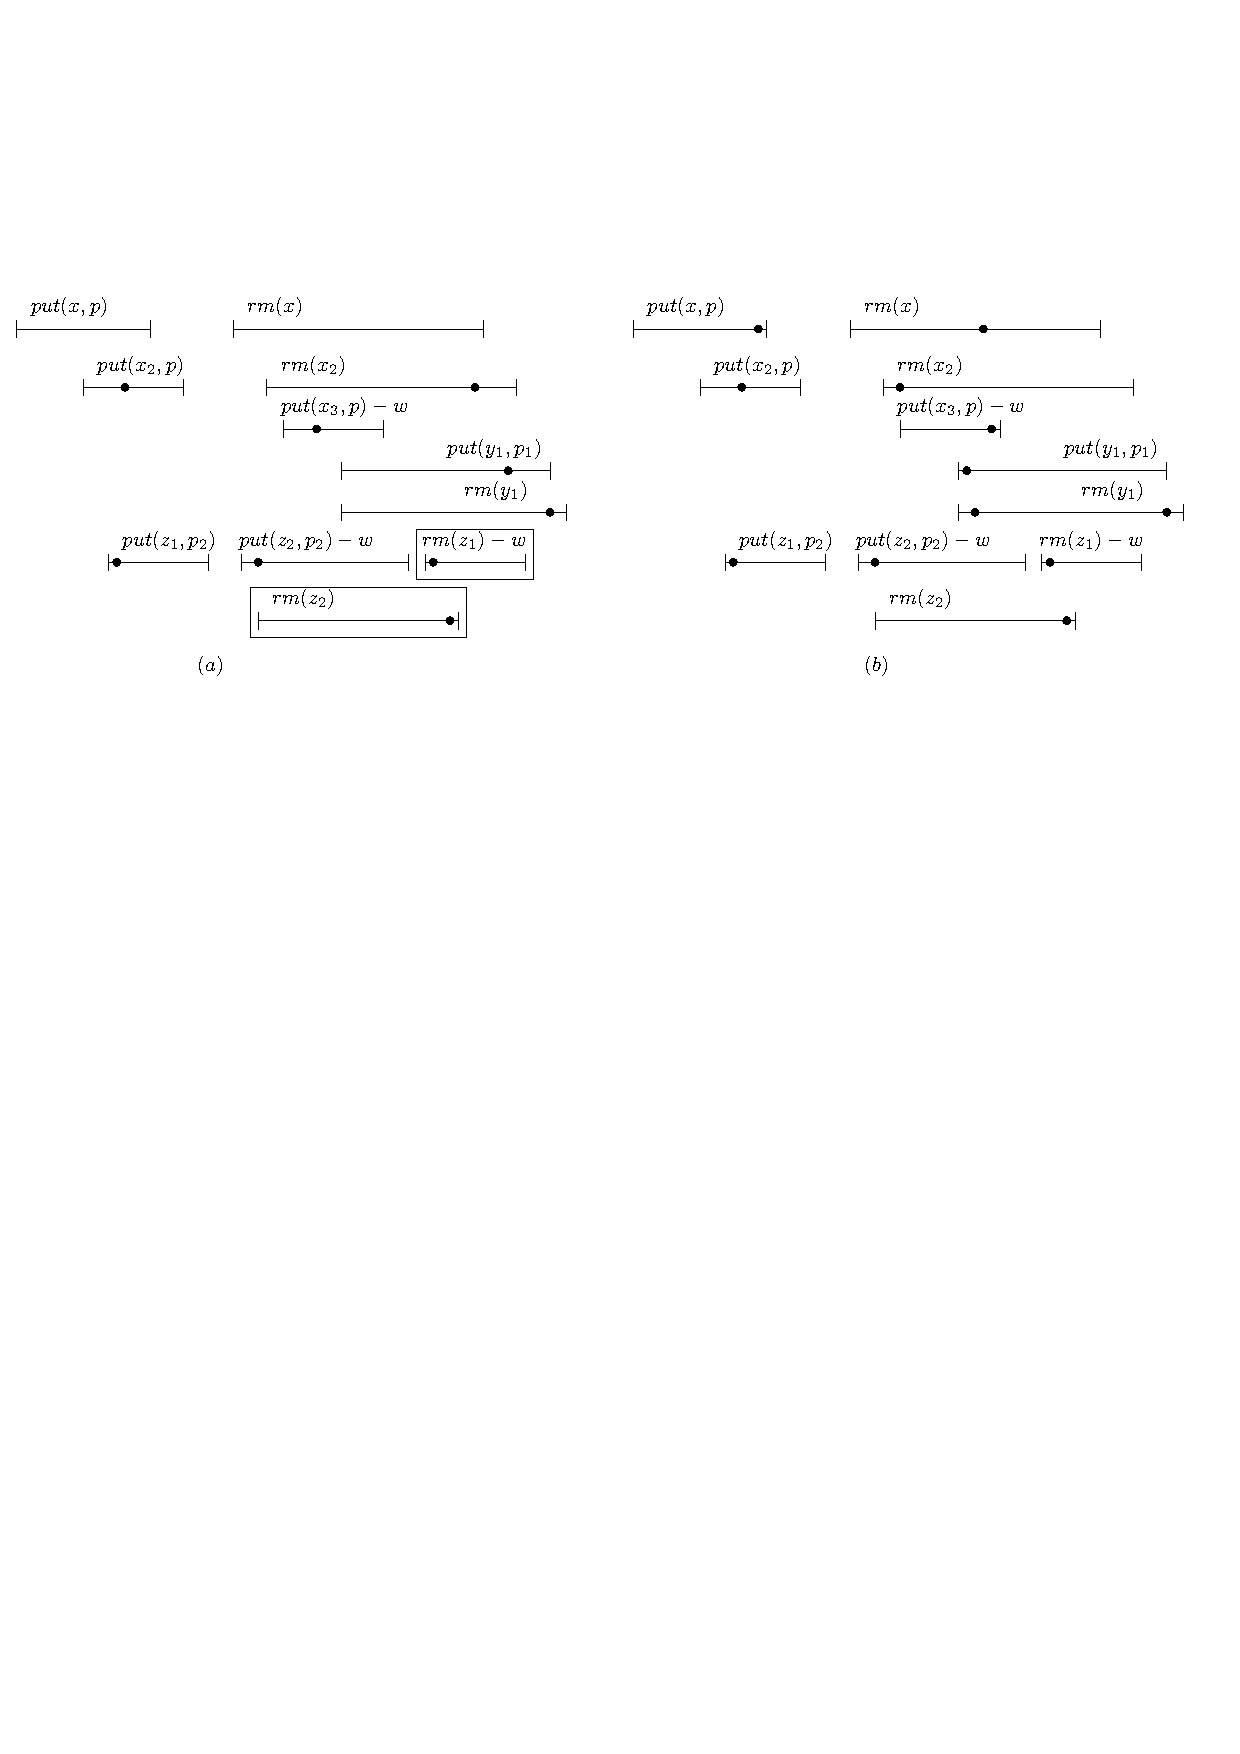
\includegraphics[width=1 \textwidth]{figures/PIC-HIS-EPQ1-TwoHis.pdf}
%\vspace{-10pt}
  \caption{The process of obtaining linearization of $e$}
  \label{fig:concurrent execution for EPQ1}
\end{figure}





